\documentclass[12pt,a4paper]{article}

\usepackage[a4paper,text={16.5cm,25.2cm},centering, margin=1in]{geometry}

\usepackage[scale=0.95]{FiraMono}
\usepackage[utf8]{inputenc}
\usepackage[T1]{fontenc}
\usepackage{mathpazo}

\usepackage{amssymb,amsmath}
\usepackage{bm}
\usepackage{graphicx}
\usepackage{microtype}
\usepackage{hyperref}
\setlength{\parindent}{0pt}
\setlength{\parskip}{1.2ex}

\usepackage{fvextra}
\DefineVerbatimEnvironment{Highlighting}{Verbatim}{breaklines,commandchars=\\\{\}}

\setcounter{secnumdepth}{0}

\hypersetup
       {   pdfauthor = { Sarah Mack (skm237) },
           pdftitle={ BEE 4750/5750 Homework 3 },
           colorlinks=TRUE,
           linkcolor=black,
           citecolor=blue,
           urlcolor=blue
       }

\title{ BEE 4750/5750 Homework 3 }

\author{ Sarah Mack (skm237) }

\date{ 2022-10-19 }

\usepackage{upquote}
\usepackage{listings}
\usepackage{xcolor}
\lstset{
    basicstyle=\ttfamily\footnotesize,
    upquote=true,
    breaklines=true,
    breakindent=0pt,
    keepspaces=true,
    showspaces=false,
    columns=fullflexible,
    showtabs=false,
    showstringspaces=false,
    escapeinside={(*@}{@*)},
    extendedchars=true,
}
\newcommand{\HLJLt}[1]{#1}
\newcommand{\HLJLw}[1]{#1}
\newcommand{\HLJLe}[1]{#1}
\newcommand{\HLJLeB}[1]{#1}
\newcommand{\HLJLo}[1]{#1}
\newcommand{\HLJLk}[1]{\textcolor[RGB]{148,91,176}{\textbf{#1}}}
\newcommand{\HLJLkc}[1]{\textcolor[RGB]{59,151,46}{\textit{#1}}}
\newcommand{\HLJLkd}[1]{\textcolor[RGB]{214,102,97}{\textit{#1}}}
\newcommand{\HLJLkn}[1]{\textcolor[RGB]{148,91,176}{\textbf{#1}}}
\newcommand{\HLJLkp}[1]{\textcolor[RGB]{148,91,176}{\textbf{#1}}}
\newcommand{\HLJLkr}[1]{\textcolor[RGB]{148,91,176}{\textbf{#1}}}
\newcommand{\HLJLkt}[1]{\textcolor[RGB]{148,91,176}{\textbf{#1}}}
\newcommand{\HLJLn}[1]{#1}
\newcommand{\HLJLna}[1]{#1}
\newcommand{\HLJLnb}[1]{#1}
\newcommand{\HLJLnbp}[1]{#1}
\newcommand{\HLJLnc}[1]{#1}
\newcommand{\HLJLncB}[1]{#1}
\newcommand{\HLJLnd}[1]{\textcolor[RGB]{214,102,97}{#1}}
\newcommand{\HLJLne}[1]{#1}
\newcommand{\HLJLneB}[1]{#1}
\newcommand{\HLJLnf}[1]{\textcolor[RGB]{66,102,213}{#1}}
\newcommand{\HLJLnfm}[1]{\textcolor[RGB]{66,102,213}{#1}}
\newcommand{\HLJLnp}[1]{#1}
\newcommand{\HLJLnl}[1]{#1}
\newcommand{\HLJLnn}[1]{#1}
\newcommand{\HLJLno}[1]{#1}
\newcommand{\HLJLnt}[1]{#1}
\newcommand{\HLJLnv}[1]{#1}
\newcommand{\HLJLnvc}[1]{#1}
\newcommand{\HLJLnvg}[1]{#1}
\newcommand{\HLJLnvi}[1]{#1}
\newcommand{\HLJLnvm}[1]{#1}
\newcommand{\HLJLl}[1]{#1}
\newcommand{\HLJLld}[1]{\textcolor[RGB]{148,91,176}{\textit{#1}}}
\newcommand{\HLJLs}[1]{\textcolor[RGB]{201,61,57}{#1}}
\newcommand{\HLJLsa}[1]{\textcolor[RGB]{201,61,57}{#1}}
\newcommand{\HLJLsb}[1]{\textcolor[RGB]{201,61,57}{#1}}
\newcommand{\HLJLsc}[1]{\textcolor[RGB]{201,61,57}{#1}}
\newcommand{\HLJLsd}[1]{\textcolor[RGB]{201,61,57}{#1}}
\newcommand{\HLJLsdB}[1]{\textcolor[RGB]{201,61,57}{#1}}
\newcommand{\HLJLsdC}[1]{\textcolor[RGB]{201,61,57}{#1}}
\newcommand{\HLJLse}[1]{\textcolor[RGB]{59,151,46}{#1}}
\newcommand{\HLJLsh}[1]{\textcolor[RGB]{201,61,57}{#1}}
\newcommand{\HLJLsi}[1]{#1}
\newcommand{\HLJLso}[1]{\textcolor[RGB]{201,61,57}{#1}}
\newcommand{\HLJLsr}[1]{\textcolor[RGB]{201,61,57}{#1}}
\newcommand{\HLJLss}[1]{\textcolor[RGB]{201,61,57}{#1}}
\newcommand{\HLJLssB}[1]{\textcolor[RGB]{201,61,57}{#1}}
\newcommand{\HLJLnB}[1]{\textcolor[RGB]{59,151,46}{#1}}
\newcommand{\HLJLnbB}[1]{\textcolor[RGB]{59,151,46}{#1}}
\newcommand{\HLJLnfB}[1]{\textcolor[RGB]{59,151,46}{#1}}
\newcommand{\HLJLnh}[1]{\textcolor[RGB]{59,151,46}{#1}}
\newcommand{\HLJLni}[1]{\textcolor[RGB]{59,151,46}{#1}}
\newcommand{\HLJLnil}[1]{\textcolor[RGB]{59,151,46}{#1}}
\newcommand{\HLJLnoB}[1]{\textcolor[RGB]{59,151,46}{#1}}
\newcommand{\HLJLoB}[1]{\textcolor[RGB]{102,102,102}{\textbf{#1}}}
\newcommand{\HLJLow}[1]{\textcolor[RGB]{102,102,102}{\textbf{#1}}}
\newcommand{\HLJLp}[1]{#1}
\newcommand{\HLJLc}[1]{\textcolor[RGB]{153,153,119}{\textit{#1}}}
\newcommand{\HLJLch}[1]{\textcolor[RGB]{153,153,119}{\textit{#1}}}
\newcommand{\HLJLcm}[1]{\textcolor[RGB]{153,153,119}{\textit{#1}}}
\newcommand{\HLJLcp}[1]{\textcolor[RGB]{153,153,119}{\textit{#1}}}
\newcommand{\HLJLcpB}[1]{\textcolor[RGB]{153,153,119}{\textit{#1}}}
\newcommand{\HLJLcs}[1]{\textcolor[RGB]{153,153,119}{\textit{#1}}}
\newcommand{\HLJLcsB}[1]{\textcolor[RGB]{153,153,119}{\textit{#1}}}
\newcommand{\HLJLg}[1]{#1}
\newcommand{\HLJLgd}[1]{#1}
\newcommand{\HLJLge}[1]{#1}
\newcommand{\HLJLgeB}[1]{#1}
\newcommand{\HLJLgh}[1]{#1}
\newcommand{\HLJLgi}[1]{#1}
\newcommand{\HLJLgo}[1]{#1}
\newcommand{\HLJLgp}[1]{#1}
\newcommand{\HLJLgs}[1]{#1}
\newcommand{\HLJLgsB}[1]{#1}
\newcommand{\HLJLgt}[1]{#1}


\begin{document}

\maketitle

%  This setups the environment and installs packages, but doesn't appear in the generated document 
%  You shouldn't need to modify this 


% - this block is hidden, but stores the generator and demand data; you can use a dataframe to combine these or refactor as you'd like 


\section{Problem 1}
\subsection{Problem 1.1}
There are three decision variables.  Generator type capacity at installation, energy production over a time period, and non-served energy over a time period. These are respectively:

\[

x_g, y_{g,t}, nse_t

\]
\subsection{Problem 1.2}
The objective function minimizes cost. The total cost includes the investment cost, the operating cost, and the non-served energy cost. The investment cost is the sum of the individual generator installation cost times its capacity. The total operating cost is the sum of the time in the period times the individual operating cost times the generation during that time period. The total non-served energy is the sum of the non-served energy cost times the non-served energy production  during that time period.

\[

\min(COST) = \sum C_g^{INV}x_g + \sum\sum L_t C_g^{OP} y_{g,t} + \sum_t C_t^{NSE} nse_t

\]
\subsection{Problem 1.3}
Generators cannot produce more than their installed capacity and availability, so the energy production over a time period must be less than or equal to the installed capacity times the capacity factor:

\[

y_{g,t} \leq x_g * CF_{g,t}

\]
Need to serve load during each time period, so the sum of the production and non-served energy production should be less than or equal to the demand:

\[

\sum (y_{g,t} + nse_{t}) \leq demand_t

\]
Installation capacity and energy production must be non-negative, which was established when the variables were created.

\subsection{Problem 1.4}

\begin{lstlisting}
(*@\HLJLnB{julia>}@*) (*@\HLJLk{using}@*) (*@\HLJLn{JuMP}@*)

(*@\HLJLnB{julia>}@*) (*@\HLJLk{using}@*) (*@\HLJLn{HiGHS}@*)

(*@\HLJLnB{julia>}@*) (*@\HLJLcs{{\#}}@*) (*@\HLJLcs{create}@*) (*@\HLJLcs{model}@*)
       (*@\HLJLn{gencap}@*) (*@\HLJLoB{=}@*) (*@\HLJLnf{Model}@*)(*@\HLJLp{(}@*)(*@\HLJLn{HiGHS}@*)(*@\HLJLoB{.}@*)(*@\HLJLn{Optimizer}@*)(*@\HLJLp{)}@*)
A JuMP Model
Feasibility problem with:
Variables: 0
Model mode: AUTOMATIC
CachingOptimizer state: EMPTY(*@{{\_}}@*)OPTIMIZER
Solver name: HiGHS

(*@\HLJLnB{julia>}@*) (*@\HLJLcs{{\#}}@*) (*@\HLJLcs{add}@*) (*@\HLJLcs{different}@*) (*@\HLJLcs{energy}@*) (*@\HLJLcs{gen}@*) (*@\HLJLcs{types}@*)
       (*@\HLJLn{generators}@*) (*@\HLJLoB{=}@*) (*@\HLJLp{[}@*)(*@\HLJLs{"{}geothermal"{}}@*)(*@\HLJLp{,}@*) (*@\HLJLs{"{}coal"{}}@*)(*@\HLJLp{,}@*) (*@\HLJLs{"{}ccgt"{}}@*)(*@\HLJLp{,}@*) (*@\HLJLs{"{}ct"{}}@*)(*@\HLJLp{,}@*) (*@\HLJLs{"{}wind"{}}@*)(*@\HLJLp{,}@*) (*@\HLJLs{"{}solar"{}}@*)(*@\HLJLp{];}@*)

(*@\HLJLnB{julia>}@*) (*@\HLJLcs{{\#}}@*) (*@\HLJLcs{variables}@*)
       (*@\HLJLn{G}@*) (*@\HLJLoB{=}@*) (*@\HLJLni{1}@*)(*@\HLJLoB{:}@*)(*@\HLJLnf{length}@*)(*@\HLJLp{(}@*)(*@\HLJLn{generators}@*)(*@\HLJLp{);}@*)

(*@\HLJLnB{julia>}@*) (*@\HLJLn{T}@*) (*@\HLJLoB{=}@*) (*@\HLJLni{1}@*)(*@\HLJLoB{:}@*)(*@\HLJLnf{length}@*)(*@\HLJLp{(}@*)(*@\HLJLn{hours}@*)(*@\HLJLp{);}@*)

(*@\HLJLnB{julia>}@*) (*@\HLJLnd{@variable}@*)(*@\HLJLp{(}@*)(*@\HLJLn{gencap}@*)(*@\HLJLp{,}@*) (*@\HLJLn{x}@*)(*@\HLJLp{[}@*)(*@\HLJLn{G}@*)(*@\HLJLp{]}@*) (*@\HLJLoB{>=}@*) (*@\HLJLni{0}@*)(*@\HLJLp{);}@*)

(*@\HLJLnB{julia>}@*) (*@\HLJLnd{@variable}@*)(*@\HLJLp{(}@*)(*@\HLJLn{gencap}@*)(*@\HLJLp{,}@*) (*@\HLJLn{y}@*)(*@\HLJLp{[}@*)(*@\HLJLn{G}@*)(*@\HLJLp{,}@*)(*@\HLJLn{T}@*)(*@\HLJLp{]}@*) (*@\HLJLoB{>=}@*) (*@\HLJLni{0}@*)(*@\HLJLp{);}@*)

(*@\HLJLnB{julia>}@*) (*@\HLJLnd{@variable}@*)(*@\HLJLp{(}@*)(*@\HLJLn{gencap}@*)(*@\HLJLp{,}@*) (*@\HLJLn{nse}@*)(*@\HLJLp{[}@*)(*@\HLJLn{T}@*)(*@\HLJLp{]}@*) (*@\HLJLoB{>=}@*) (*@\HLJLni{0}@*)(*@\HLJLp{);}@*)

(*@\HLJLnB{julia>}@*) (*@\HLJLcs{{\#}}@*) (*@\HLJLcs{create}@*) (*@\HLJLcs{objective}@*) (*@\HLJLcs{function}@*)
       (*@\HLJLnd{@objective}@*)(*@\HLJLp{(}@*)(*@\HLJLn{gencap}@*)(*@\HLJLp{,}@*) (*@\HLJLn{Min}@*)(*@\HLJLp{,}@*) (*@\HLJLn{investment{\_}cost}@*)(*@\HLJLoB{{\textquotesingle}*}@*)(*@\HLJLn{x}@*) (*@\HLJLoB{+}@*) (*@\HLJLnf{sum}@*)(*@\HLJLp{(}@*)(*@\HLJLn{op{\_}cost}@*)(*@\HLJLoB{.*}@*)(*@\HLJLn{y}@*)(*@\HLJLp{)}@*)(*@\HLJLoB{*}@*)(*@\HLJLni{365}@*) (*@\HLJLoB{+}@*) (*@\HLJLni{1000}@*)(*@\HLJLoB{*}@*)(*@\HLJLnf{sum}@*)(*@\HLJLp{(}@*)(*@\HLJLn{nse}@*)(*@\HLJLp{)}@*)(*@\HLJLoB{*}@*)(*@\HLJLni{365}@*)(*@\HLJLp{);}@*)

(*@\HLJLnB{julia>}@*) (*@\HLJLcs{{\#}}@*) (*@\HLJLcs{generators}@*) (*@\HLJLcs{cannot}@*) (*@\HLJLcs{produce}@*) (*@\HLJLcs{more}@*) (*@\HLJLcs{than}@*) (*@\HLJLcs{their}@*) (*@\HLJLcs{installed}@*) (*@\HLJLcs{capacity}@*) (*@\HLJLcs{and}@*) (*@\HLJLcs{availability}@*)
       (*@\HLJLn{avail}@*) (*@\HLJLoB{=}@*) (*@\HLJLnf{zeros}@*)(*@\HLJLp{(}@*)(*@\HLJLnf{length}@*)(*@\HLJLp{(}@*)(*@\HLJLn{G}@*)(*@\HLJLp{),}@*) (*@\HLJLnf{length}@*)(*@\HLJLp{(}@*)(*@\HLJLn{T}@*)(*@\HLJLp{));}@*)

(*@\HLJLnB{julia>}@*) (*@\HLJLn{avail}@*)(*@\HLJLp{[}@*)(*@\HLJLni{1}@*)(*@\HLJLp{,}@*)(*@\HLJLoB{:}@*)(*@\HLJLp{]}@*) (*@\HLJLoB{=}@*) (*@\HLJLn{thermal{\_}cf}@*)(*@\HLJLp{[}@*)(*@\HLJLni{1}@*)(*@\HLJLp{]}@*)(*@\HLJLoB{*}@*)(*@\HLJLnf{ones}@*)(*@\HLJLp{(}@*)(*@\HLJLnf{length}@*)(*@\HLJLp{(}@*)(*@\HLJLn{T}@*)(*@\HLJLp{));}@*)

(*@\HLJLnB{julia>}@*) (*@\HLJLn{avail}@*)(*@\HLJLp{[}@*)(*@\HLJLni{2}@*)(*@\HLJLp{,}@*)(*@\HLJLoB{:}@*)(*@\HLJLp{]}@*) (*@\HLJLoB{=}@*) (*@\HLJLn{thermal{\_}cf}@*)(*@\HLJLp{[}@*)(*@\HLJLni{2}@*)(*@\HLJLp{]}@*)(*@\HLJLoB{*}@*)(*@\HLJLnf{ones}@*)(*@\HLJLp{(}@*)(*@\HLJLnf{length}@*)(*@\HLJLp{(}@*)(*@\HLJLn{T}@*)(*@\HLJLp{));}@*)

(*@\HLJLnB{julia>}@*) (*@\HLJLn{avail}@*)(*@\HLJLp{[}@*)(*@\HLJLni{3}@*)(*@\HLJLp{,}@*)(*@\HLJLoB{:}@*)(*@\HLJLp{]}@*) (*@\HLJLoB{=}@*) (*@\HLJLn{thermal{\_}cf}@*)(*@\HLJLp{[}@*)(*@\HLJLni{3}@*)(*@\HLJLp{]}@*)(*@\HLJLoB{*}@*)(*@\HLJLnf{ones}@*)(*@\HLJLp{(}@*)(*@\HLJLnf{length}@*)(*@\HLJLp{(}@*)(*@\HLJLn{T}@*)(*@\HLJLp{));}@*)

(*@\HLJLnB{julia>}@*) (*@\HLJLn{avail}@*)(*@\HLJLp{[}@*)(*@\HLJLni{4}@*)(*@\HLJLp{,}@*)(*@\HLJLoB{:}@*)(*@\HLJLp{]}@*) (*@\HLJLoB{=}@*) (*@\HLJLn{thermal{\_}cf}@*)(*@\HLJLp{[}@*)(*@\HLJLni{4}@*)(*@\HLJLp{]}@*)(*@\HLJLoB{*}@*)(*@\HLJLnf{ones}@*)(*@\HLJLp{(}@*)(*@\HLJLnf{length}@*)(*@\HLJLp{(}@*)(*@\HLJLn{T}@*)(*@\HLJLp{));}@*)

(*@\HLJLnB{julia>}@*) (*@\HLJLn{avail}@*)(*@\HLJLp{[}@*)(*@\HLJLni{5}@*)(*@\HLJLp{,}@*)(*@\HLJLoB{:}@*)(*@\HLJLp{]}@*) (*@\HLJLoB{=}@*) (*@\HLJLn{wind{\_}cf}@*)(*@\HLJLp{;}@*)

(*@\HLJLnB{julia>}@*) (*@\HLJLn{avail}@*)(*@\HLJLp{[}@*)(*@\HLJLni{6}@*)(*@\HLJLp{,}@*)(*@\HLJLoB{:}@*)(*@\HLJLp{]}@*) (*@\HLJLoB{=}@*) (*@\HLJLn{solar{\_}cf}@*)(*@\HLJLp{;}@*)

(*@\HLJLnB{julia>}@*) (*@\HLJLnd{@constraint}@*)(*@\HLJLp{(}@*)(*@\HLJLn{gencap}@*)(*@\HLJLp{,}@*) (*@\HLJLn{availability}@*)(*@\HLJLp{[}@*)(*@\HLJLn{g}@*) (*@\HLJLkp{in}@*) (*@\HLJLn{G}@*)(*@\HLJLp{,}@*) (*@\HLJLn{t}@*) (*@\HLJLkp{in}@*) (*@\HLJLn{T}@*)(*@\HLJLp{],}@*) (*@\HLJLn{y}@*)(*@\HLJLp{[}@*)(*@\HLJLn{g}@*)(*@\HLJLp{,}@*) (*@\HLJLn{t}@*)(*@\HLJLp{]}@*) (*@\HLJLoB{<=}@*) (*@\HLJLn{avail}@*)(*@\HLJLp{[}@*)(*@\HLJLn{g}@*)(*@\HLJLp{,}@*) (*@\HLJLn{t}@*)(*@\HLJLp{]}@*) (*@\HLJLoB{*}@*) (*@\HLJLn{x}@*)(*@\HLJLp{[}@*)(*@\HLJLn{g}@*)(*@\HLJLp{]);}@*)

(*@\HLJLnB{julia>}@*) (*@\HLJLcs{{\#}}@*) (*@\HLJLcs{need}@*) (*@\HLJLcs{to}@*) (*@\HLJLcs{serve}@*) (*@\HLJLcs{load}@*) (*@\HLJLcs{during}@*) (*@\HLJLcs{each}@*) (*@\HLJLcs{time}@*) (*@\HLJLcs{period}@*)
       (*@\HLJLnd{@constraint}@*)(*@\HLJLp{(}@*)(*@\HLJLn{gencap}@*)(*@\HLJLp{,}@*) (*@\HLJLn{load}@*)(*@\HLJLp{[}@*)(*@\HLJLn{t}@*) (*@\HLJLkp{in}@*) (*@\HLJLn{T}@*)(*@\HLJLp{],}@*) (*@\HLJLnf{sum}@*)(*@\HLJLp{(}@*)(*@\HLJLn{y}@*)(*@\HLJLp{[}@*)(*@\HLJLoB{:}@*)(*@\HLJLp{,}@*)(*@\HLJLn{t}@*)(*@\HLJLp{])}@*) (*@\HLJLoB{+}@*) (*@\HLJLn{nse}@*)(*@\HLJLp{[}@*)(*@\HLJLn{t}@*)(*@\HLJLp{]}@*) (*@\HLJLoB{==}@*) (*@\HLJLn{demand}@*)(*@\HLJLp{[}@*)(*@\HLJLn{t}@*)(*@\HLJLp{])}@*);
\end{lstlisting}

\subsection{Problem 1.5}

\begin{lstlisting}
(*@\HLJLnB{julia>}@*) (*@\HLJLcs{{\#}}@*) (*@\HLJLcs{optimize}@*) (*@\HLJLcs{model}@*)
       (*@\HLJLnf{optimize!}@*)(*@\HLJLp{(}@*)(*@\HLJLn{gencap}@*)(*@\HLJLp{)}@*)
Presolving model
156 rows, 162 cols, 420 nonzeros
156 rows, 162 cols, 420 nonzeros
Presolve : Reductions: rows 156(-12); columns 162(-12); elements 420(-24)
Solving the presolved LP
Using EKK dual simplex solver - serial
  Iteration        Objective     Infeasibilities num(sum)
          0     0.0000000000e+00 Pr: 24(60321.5) 0s
        120     9.1214221224e+08 Pr: 0(0) 0s
Solving the original LP from the solution after postsolve
Model   status      : Optimal
Simplex   iterations: 120
Objective value     :  9.1214221224e+08
HiGHS run time      :          0.00

(*@\HLJLnB{julia>}@*) (*@\HLJLnf{objective{\_}value}@*)(*@\HLJLp{(}@*)(*@\HLJLn{gencap}@*)(*@\HLJLp{)}@*)
9.12142212241888e8

(*@\HLJLnB{julia>}@*) (*@\HLJLn{value}@*)(*@\HLJLoB{.}@*)(*@\HLJLp{(}@*)(*@\HLJLn{x}@*)(*@\HLJLp{)}@*)
1-dimensional DenseAxisArray(*@{{\{}}@*)Float64,1,...(*@{{\}}}@*) with index sets:
    Dimension 1, 1:6
And data, a 6-element Vector(*@{{\{}}@*)Float64(*@{{\}}}@*):
    0.0
    0.0
 1704.2566371681414
  881.3274336283189
 1238.053097345133
 2728.9085545722714

(*@\HLJLnB{julia>}@*) (*@\HLJLn{value}@*)(*@\HLJLoB{.}@*)(*@\HLJLp{(}@*)(*@\HLJLn{y}@*)(*@\HLJLp{)}@*)
2-dimensional DenseAxisArray(*@{{\{}}@*)Float64,2,...(*@{{\}}}@*) with index sets:
    Dimension 1, 1:6
    Dimension 2, 1:24
And data, a 6(*@\ensuremath{\times}@*)24 Matrix(*@{{\{}}@*)Float64(*@{{\}}}@*):
  -0.0     -0.0    -0.0      -0.0      -0.0    (*@\ensuremath{\ldots}@*)    -0.0     -0.0     -0.0
  -0.0     -0.0    -0.0      -0.0      -0.0         -0.0     -0.0     -0.0
 798.929  780.31  863.071  1386.35   1704.26      1227.31  1003.07   844.929
   0.0      0.0     0.0       0.0     180.416        0.0      0.0      0.0
 718.071  705.69  680.929   346.655   173.327      705.69   680.929  718.071
  -0.0     -0.0    -0.0      -0.0      -0.0    (*@\ensuremath{\ldots}@*)    -0.0     -0.0     -0.0

(*@\HLJLnB{julia>}@*) (*@\HLJLn{value}@*)(*@\HLJLoB{.}@*)(*@\HLJLp{(}@*)(*@\HLJLn{nse}@*)(*@\HLJLp{)}@*)
1-dimensional DenseAxisArray(*@{{\{}}@*)Float64,1,...(*@{{\}}}@*) with index sets:
    Dimension 1, 1:24
And data, a 24-element Vector(*@{{\{}}@*)Float64(*@{{\}}}@*):
 0.0
 0.0
 0.0
 0.0
 0.0
 0.0
 0.0
 0.0
 0.0
 0.0
 (*@\ensuremath{\vdots}@*)
 0.0
 0.0
 0.0
 0.0
 0.0
 0.0
 0.0
 0.0
 0.0
\end{lstlisting}

The cost of the optimized model is \$ 912,142,212. The installation plan is detailed in the table below. The non-served energy is always 0.


\begin{lstlisting}
(*@\HLJLnB{julia>}@*) (*@\HLJLk{using}@*) (*@\HLJLn{DataFrames}@*)

(*@\HLJLnB{julia>}@*) (*@\HLJLn{results}@*) (*@\HLJLoB{=}@*) (*@\HLJLnf{DataFrame}@*)(*@\HLJLp{(}@*)
                   (*@\HLJLs{"{}Generation}@*) (*@\HLJLs{Type"{}}@*)        (*@\HLJLoB{=>}@*) (*@\HLJLn{generators}@*)(*@\HLJLp{,}@*)
                   (*@\HLJLs{"{}Installed}@*) (*@\HLJLs{MW"{}}@*)  (*@\HLJLoB{=>}@*) (*@\HLJLn{value}@*)(*@\HLJLoB{.}@*)(*@\HLJLp{(}@*)(*@\HLJLn{x}@*)(*@\HLJLp{)}@*)(*@\HLJLoB{.}@*)(*@\HLJLn{data}@*)(*@\HLJLp{,}@*)
                   (*@\HLJLp{)}@*)
6(*@\ensuremath{\times}@*)2 DataFrame
 Row │ Generation Type  Installed MW
     │ String           Float64
─────┼───────────────────────────────
   1 │ geothermal              0.0
   2 │ coal                    0.0
   3 │ ccgt                 1704.26
   4 │ ct                    881.327
   5 │ wind                 1238.05
   6 │ solar                2728.91
\end{lstlisting}

\subsection{Problem 1.6}

\begin{lstlisting}
(*@\HLJLnB{julia>}@*) (*@\HLJLk{using}@*) (*@\HLJLn{Plots}@*)

(*@\HLJLnB{julia>}@*) (*@\HLJLcs{{\#}}@*) (*@\HLJLcs{create}@*) (*@\HLJLcs{array}@*) (*@\HLJLcs{for}@*) (*@\HLJLcs{plotting}@*) (*@\HLJLcs{loads}@*) (*@\HLJLcs{over}@*) (*@\HLJLcs{a}@*) (*@\HLJLcs{24}@*) (*@\HLJLcs{hr}@*) (*@\HLJLcs{period}@*)
       (*@\HLJLn{loads}@*) (*@\HLJLoB{=}@*) (*@\HLJLn{value}@*)(*@\HLJLoB{.}@*)(*@\HLJLp{(}@*)(*@\HLJLn{y}@*)(*@\HLJLp{)}@*)(*@\HLJLoB{.}@*)(*@\HLJLn{data}@*)(*@\HLJLp{;}@*)

(*@\HLJLnB{julia>}@*) (*@\HLJLcs{{\#}}@*) (*@\HLJLcs{plot}@*) (*@\HLJLcs{line}@*) (*@\HLJLcs{plot}@*)
       (*@\HLJLnf{plot}@*)(*@\HLJLp{(}@*)(*@\HLJLn{loads}@*)(*@\HLJLoB{{\textquotesingle}}@*)(*@\HLJLp{,}@*) (*@\HLJLn{label}@*)(*@\HLJLoB{=}@*)(*@\HLJLnf{permutedims}@*)(*@\HLJLp{([}@*)(*@\HLJLs{"{}geothermal"{}}@*)(*@\HLJLp{,}@*)(*@\HLJLs{"{}coal"{}}@*)(*@\HLJLp{,}@*)(*@\HLJLs{"{}ccgt"{}}@*)(*@\HLJLp{,}@*)(*@\HLJLs{"{}ct"{}}@*)(*@\HLJLp{,}@*)(*@\HLJLs{"{}wind"{}}@*)(*@\HLJLp{,}@*)(*@\HLJLs{"{}solar"{}}@*)(*@\HLJLp{]),}@*) (*@\HLJLn{title}@*)(*@\HLJLoB{=}@*)(*@\HLJLs{"{}Energy}@*) (*@\HLJLs{Gen}@*) (*@\HLJLs{over}@*) (*@\HLJLs{24}@*) (*@\HLJLs{hr"{}}@*)(*@\HLJLp{,}@*) (*@\HLJLn{xlabel}@*)(*@\HLJLoB{=}@*)(*@\HLJLs{"{}Hr"{}}@*)(*@\HLJLp{,}@*) (*@\HLJLn{ylabel}@*)(*@\HLJLoB{=}@*)(*@\HLJLs{"{}MW"{}}@*))
\end{lstlisting}
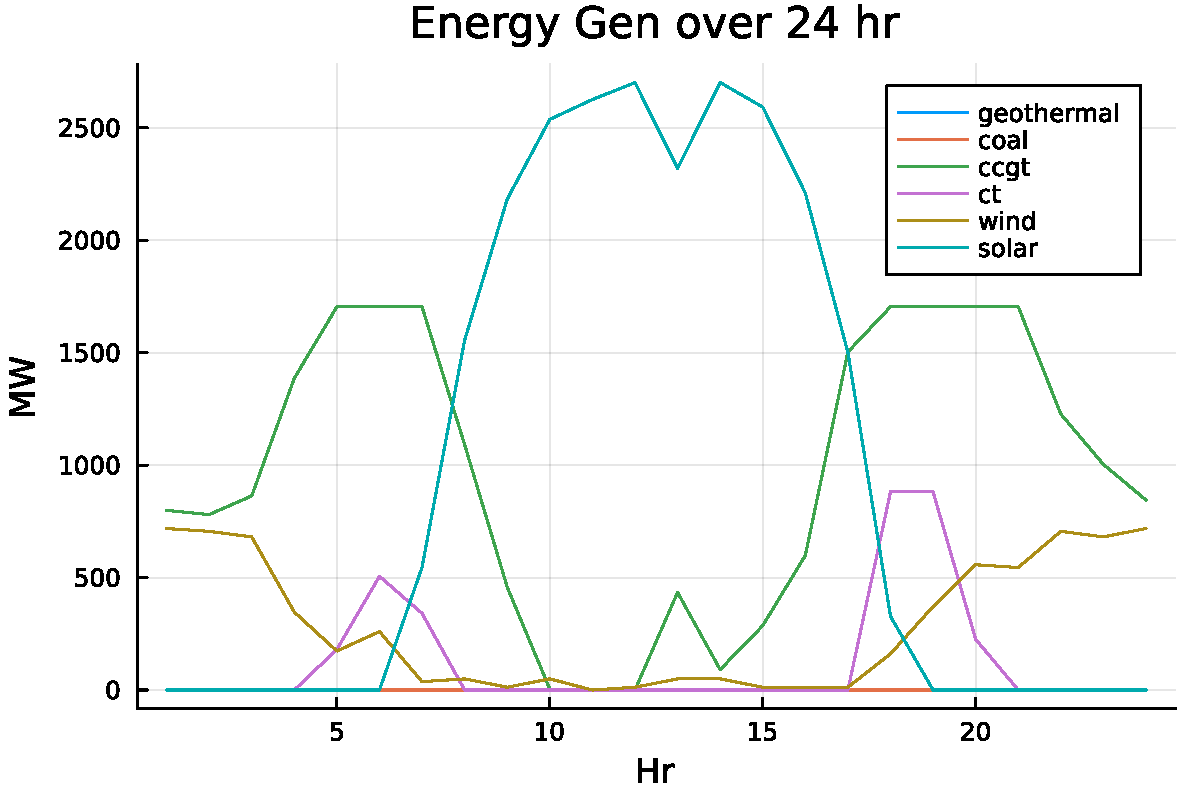
\includegraphics[width=\linewidth]{figures/solution-template_6_1.pdf}

\begin{lstlisting}
(*@\HLJLnB{julia>}@*) (*@\HLJLcs{{\#}}@*) (*@\HLJLcs{plot}@*) (*@\HLJLcs{stacked}@*) (*@\HLJLcs{area}@*) (*@\HLJLcs{plot}@*)
       (*@\HLJLnf{areaplot}@*)(*@\HLJLp{(}@*)(*@\HLJLn{loads}@*)(*@\HLJLoB{{\textquotesingle}}@*)(*@\HLJLp{,}@*) (*@\HLJLn{label}@*)(*@\HLJLoB{=}@*)(*@\HLJLnf{permutedims}@*)(*@\HLJLp{([}@*)(*@\HLJLs{"{}geothermal"{}}@*)(*@\HLJLp{,}@*)(*@\HLJLs{"{}coal"{}}@*)(*@\HLJLp{,}@*)(*@\HLJLs{"{}ccgt"{}}@*)(*@\HLJLp{,}@*)(*@\HLJLs{"{}ct"{}}@*)(*@\HLJLp{,}@*)(*@\HLJLs{"{}wind"{}}@*)(*@\HLJLp{,}@*)(*@\HLJLs{"{}solar"{}}@*)(*@\HLJLp{]),}@*) (*@\HLJLn{title}@*)(*@\HLJLoB{=}@*)(*@\HLJLs{"{}Energy}@*) (*@\HLJLs{Gen}@*) (*@\HLJLs{over}@*) (*@\HLJLs{24}@*) (*@\HLJLs{hr"{}}@*)(*@\HLJLp{,}@*) (*@\HLJLn{xlabel}@*)(*@\HLJLoB{=}@*)(*@\HLJLs{"{}Hr"{}}@*)(*@\HLJLp{,}@*) (*@\HLJLn{ylabel}@*)(*@\HLJLoB{=}@*)(*@\HLJLs{"{}MW"{}}@*))
\end{lstlisting}
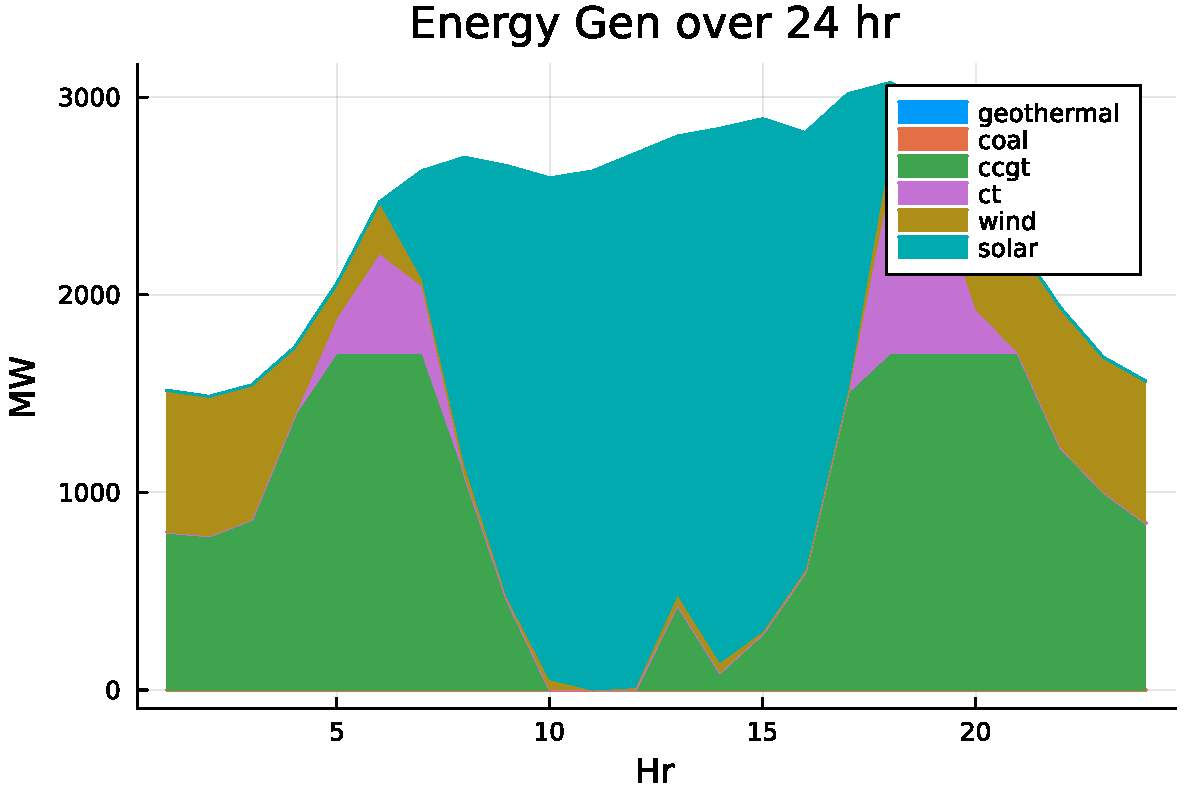
\includegraphics[width=\linewidth]{figures/solution-template_6_2.pdf}

Solar energy is the main draw during the sunny hours of the day, with CT and CCGT kicking in during the transitional hours.  Wind and CCGT are the main contributors in the nighttime.

\section{Problem 2}
\subsection{Problem 2.1}
The only change that needs to be added is the inclusion of another constraint. This must include the emission limit  of 1.5 MtCO2/yr. Therefore the emissions times the sum of generation times 365 days cannot exceed the emission limit.

\[

\sum (y_{g,t}) * e_g * 365 \leq 1.5 \text{ MtCO2}

\]
\subsection{Problem 2.2}

\begin{lstlisting}
(*@\HLJLnB{julia>}@*) (*@\HLJLcs{{\#}}@*) (*@\HLJLcs{create}@*) (*@\HLJLcs{new}@*) (*@\HLJLcs{model}@*)
       (*@\HLJLn{gencap2}@*) (*@\HLJLoB{=}@*) (*@\HLJLnf{Model}@*)(*@\HLJLp{(}@*)(*@\HLJLn{HiGHS}@*)(*@\HLJLoB{.}@*)(*@\HLJLn{Optimizer}@*)(*@\HLJLp{)}@*)
A JuMP Model
Feasibility problem with:
Variables: 0
Model mode: AUTOMATIC
CachingOptimizer state: EMPTY(*@{{\_}}@*)OPTIMIZER
Solver name: HiGHS

(*@\HLJLnB{julia>}@*) (*@\HLJLcs{{\#}}@*) (*@\HLJLcs{add}@*) (*@\HLJLcs{different}@*) (*@\HLJLcs{energy}@*) (*@\HLJLcs{gen}@*) (*@\HLJLcs{types}@*)
       (*@\HLJLn{generators}@*) (*@\HLJLoB{=}@*) (*@\HLJLp{[}@*)(*@\HLJLs{"{}geothermal"{}}@*)(*@\HLJLp{,}@*) (*@\HLJLs{"{}coal"{}}@*)(*@\HLJLp{,}@*) (*@\HLJLs{"{}ccgt"{}}@*)(*@\HLJLp{,}@*) (*@\HLJLs{"{}ct"{}}@*)(*@\HLJLp{,}@*) (*@\HLJLs{"{}wind"{}}@*)(*@\HLJLp{,}@*) (*@\HLJLs{"{}solar"{}}@*)(*@\HLJLp{];}@*)

(*@\HLJLnB{julia>}@*) (*@\HLJLcs{{\#}}@*) (*@\HLJLcs{variables}@*)
       (*@\HLJLn{G}@*) (*@\HLJLoB{=}@*) (*@\HLJLni{1}@*)(*@\HLJLoB{:}@*)(*@\HLJLnf{length}@*)(*@\HLJLp{(}@*)(*@\HLJLn{generators}@*)(*@\HLJLp{);}@*)

(*@\HLJLnB{julia>}@*) (*@\HLJLn{T}@*) (*@\HLJLoB{=}@*) (*@\HLJLni{1}@*)(*@\HLJLoB{:}@*)(*@\HLJLnf{length}@*)(*@\HLJLp{(}@*)(*@\HLJLn{hours}@*)(*@\HLJLp{);}@*)

(*@\HLJLnB{julia>}@*) (*@\HLJLnd{@variable}@*)(*@\HLJLp{(}@*)(*@\HLJLn{gencap2}@*)(*@\HLJLp{,}@*) (*@\HLJLn{x}@*)(*@\HLJLp{[}@*)(*@\HLJLn{G}@*)(*@\HLJLp{]}@*) (*@\HLJLoB{>=}@*) (*@\HLJLni{0}@*)(*@\HLJLp{);}@*)

(*@\HLJLnB{julia>}@*) (*@\HLJLnd{@variable}@*)(*@\HLJLp{(}@*)(*@\HLJLn{gencap2}@*)(*@\HLJLp{,}@*) (*@\HLJLn{y}@*)(*@\HLJLp{[}@*)(*@\HLJLn{G}@*)(*@\HLJLp{,}@*)(*@\HLJLn{T}@*)(*@\HLJLp{]}@*) (*@\HLJLoB{>=}@*) (*@\HLJLni{0}@*)(*@\HLJLp{);}@*)

(*@\HLJLnB{julia>}@*) (*@\HLJLnd{@variable}@*)(*@\HLJLp{(}@*)(*@\HLJLn{gencap2}@*)(*@\HLJLp{,}@*) (*@\HLJLn{nse}@*)(*@\HLJLp{[}@*)(*@\HLJLn{T}@*)(*@\HLJLp{]}@*) (*@\HLJLoB{>=}@*) (*@\HLJLni{0}@*)(*@\HLJLp{);}@*)

(*@\HLJLnB{julia>}@*) (*@\HLJLcs{{\#}}@*) (*@\HLJLcs{create}@*) (*@\HLJLcs{objective}@*) (*@\HLJLcs{function}@*)
       (*@\HLJLnd{@objective}@*)(*@\HLJLp{(}@*)(*@\HLJLn{gencap2}@*)(*@\HLJLp{,}@*) (*@\HLJLn{Min}@*)(*@\HLJLp{,}@*) (*@\HLJLn{investment{\_}cost}@*)(*@\HLJLoB{{\textquotesingle}*}@*)(*@\HLJLn{x}@*) (*@\HLJLoB{+}@*) (*@\HLJLnf{sum}@*)(*@\HLJLp{(}@*)(*@\HLJLn{op{\_}cost}@*)(*@\HLJLoB{.*}@*)(*@\HLJLn{y}@*)(*@\HLJLp{)}@*)(*@\HLJLoB{*}@*)(*@\HLJLni{365}@*) (*@\HLJLoB{+}@*) (*@\HLJLni{1000}@*)(*@\HLJLoB{*}@*)(*@\HLJLnf{sum}@*)(*@\HLJLp{(}@*)(*@\HLJLn{nse}@*)(*@\HLJLp{)}@*)(*@\HLJLoB{*}@*)(*@\HLJLni{365}@*)(*@\HLJLp{);}@*)

(*@\HLJLnB{julia>}@*) (*@\HLJLcs{{\#}}@*) (*@\HLJLcs{generators}@*) (*@\HLJLcs{cannot}@*) (*@\HLJLcs{produce}@*) (*@\HLJLcs{more}@*) (*@\HLJLcs{than}@*) (*@\HLJLcs{their}@*) (*@\HLJLcs{installed}@*) (*@\HLJLcs{capacity}@*) (*@\HLJLcs{and}@*) (*@\HLJLcs{availability}@*)
       (*@\HLJLn{avail}@*) (*@\HLJLoB{=}@*) (*@\HLJLnf{zeros}@*)(*@\HLJLp{(}@*)(*@\HLJLnf{length}@*)(*@\HLJLp{(}@*)(*@\HLJLn{G}@*)(*@\HLJLp{),}@*) (*@\HLJLnf{length}@*)(*@\HLJLp{(}@*)(*@\HLJLn{T}@*)(*@\HLJLp{));}@*)

(*@\HLJLnB{julia>}@*) (*@\HLJLn{avail}@*)(*@\HLJLp{[}@*)(*@\HLJLni{1}@*)(*@\HLJLp{,}@*)(*@\HLJLoB{:}@*)(*@\HLJLp{]}@*) (*@\HLJLoB{=}@*) (*@\HLJLn{thermal{\_}cf}@*)(*@\HLJLp{[}@*)(*@\HLJLni{1}@*)(*@\HLJLp{]}@*)(*@\HLJLoB{*}@*)(*@\HLJLnf{ones}@*)(*@\HLJLp{(}@*)(*@\HLJLnf{length}@*)(*@\HLJLp{(}@*)(*@\HLJLn{T}@*)(*@\HLJLp{));}@*)

(*@\HLJLnB{julia>}@*) (*@\HLJLn{avail}@*)(*@\HLJLp{[}@*)(*@\HLJLni{2}@*)(*@\HLJLp{,}@*)(*@\HLJLoB{:}@*)(*@\HLJLp{]}@*) (*@\HLJLoB{=}@*) (*@\HLJLn{thermal{\_}cf}@*)(*@\HLJLp{[}@*)(*@\HLJLni{2}@*)(*@\HLJLp{]}@*)(*@\HLJLoB{*}@*)(*@\HLJLnf{ones}@*)(*@\HLJLp{(}@*)(*@\HLJLnf{length}@*)(*@\HLJLp{(}@*)(*@\HLJLn{T}@*)(*@\HLJLp{));}@*)

(*@\HLJLnB{julia>}@*) (*@\HLJLn{avail}@*)(*@\HLJLp{[}@*)(*@\HLJLni{3}@*)(*@\HLJLp{,}@*)(*@\HLJLoB{:}@*)(*@\HLJLp{]}@*) (*@\HLJLoB{=}@*) (*@\HLJLn{thermal{\_}cf}@*)(*@\HLJLp{[}@*)(*@\HLJLni{3}@*)(*@\HLJLp{]}@*)(*@\HLJLoB{*}@*)(*@\HLJLnf{ones}@*)(*@\HLJLp{(}@*)(*@\HLJLnf{length}@*)(*@\HLJLp{(}@*)(*@\HLJLn{T}@*)(*@\HLJLp{));}@*)

(*@\HLJLnB{julia>}@*) (*@\HLJLn{avail}@*)(*@\HLJLp{[}@*)(*@\HLJLni{4}@*)(*@\HLJLp{,}@*)(*@\HLJLoB{:}@*)(*@\HLJLp{]}@*) (*@\HLJLoB{=}@*) (*@\HLJLn{thermal{\_}cf}@*)(*@\HLJLp{[}@*)(*@\HLJLni{4}@*)(*@\HLJLp{]}@*)(*@\HLJLoB{*}@*)(*@\HLJLnf{ones}@*)(*@\HLJLp{(}@*)(*@\HLJLnf{length}@*)(*@\HLJLp{(}@*)(*@\HLJLn{T}@*)(*@\HLJLp{));}@*)

(*@\HLJLnB{julia>}@*) (*@\HLJLn{avail}@*)(*@\HLJLp{[}@*)(*@\HLJLni{5}@*)(*@\HLJLp{,}@*)(*@\HLJLoB{:}@*)(*@\HLJLp{]}@*) (*@\HLJLoB{=}@*) (*@\HLJLn{wind{\_}cf}@*)(*@\HLJLp{;}@*)

(*@\HLJLnB{julia>}@*) (*@\HLJLn{avail}@*)(*@\HLJLp{[}@*)(*@\HLJLni{6}@*)(*@\HLJLp{,}@*)(*@\HLJLoB{:}@*)(*@\HLJLp{]}@*) (*@\HLJLoB{=}@*) (*@\HLJLn{solar{\_}cf}@*)(*@\HLJLp{;}@*)

(*@\HLJLnB{julia>}@*) (*@\HLJLnd{@constraint}@*)(*@\HLJLp{(}@*)(*@\HLJLn{gencap2}@*)(*@\HLJLp{,}@*) (*@\HLJLn{availability}@*)(*@\HLJLp{[}@*)(*@\HLJLn{g}@*) (*@\HLJLkp{in}@*) (*@\HLJLn{G}@*)(*@\HLJLp{,}@*) (*@\HLJLn{t}@*) (*@\HLJLkp{in}@*) (*@\HLJLn{T}@*)(*@\HLJLp{],}@*) (*@\HLJLn{y}@*)(*@\HLJLp{[}@*)(*@\HLJLn{g}@*)(*@\HLJLp{,}@*) (*@\HLJLn{t}@*)(*@\HLJLp{]}@*) (*@\HLJLoB{<=}@*) (*@\HLJLn{avail}@*)(*@\HLJLp{[}@*)(*@\HLJLn{g}@*)(*@\HLJLp{,}@*) (*@\HLJLn{t}@*)(*@\HLJLp{]}@*) (*@\HLJLoB{*}@*) (*@\HLJLn{x}@*)(*@\HLJLp{[}@*)(*@\HLJLn{g}@*)(*@\HLJLp{]);}@*)

(*@\HLJLnB{julia>}@*) (*@\HLJLcs{{\#}}@*) (*@\HLJLcs{need}@*) (*@\HLJLcs{to}@*) (*@\HLJLcs{serve}@*) (*@\HLJLcs{load}@*) (*@\HLJLcs{during}@*) (*@\HLJLcs{each}@*) (*@\HLJLcs{time}@*) (*@\HLJLcs{period}@*)
       (*@\HLJLnd{@constraint}@*)(*@\HLJLp{(}@*)(*@\HLJLn{gencap2}@*)(*@\HLJLp{,}@*) (*@\HLJLn{load}@*)(*@\HLJLp{[}@*)(*@\HLJLn{t}@*) (*@\HLJLkp{in}@*) (*@\HLJLn{T}@*)(*@\HLJLp{],}@*) (*@\HLJLnf{sum}@*)(*@\HLJLp{(}@*)(*@\HLJLn{y}@*)(*@\HLJLp{[}@*)(*@\HLJLoB{:}@*)(*@\HLJLp{,}@*)(*@\HLJLn{t}@*)(*@\HLJLp{])}@*) (*@\HLJLoB{+}@*) (*@\HLJLn{nse}@*)(*@\HLJLp{[}@*)(*@\HLJLn{t}@*)(*@\HLJLp{]}@*) (*@\HLJLoB{==}@*) (*@\HLJLn{demand}@*)(*@\HLJLp{[}@*)(*@\HLJLn{t}@*)(*@\HLJLp{]);}@*)

(*@\HLJLnB{julia>}@*) (*@\HLJLcs{{\#}}@*) (*@\HLJLcs{new}@*) (*@\HLJLcs{emissions}@*) (*@\HLJLcs{constraint}@*)
       (*@\HLJLnd{@constraint}@*)(*@\HLJLp{(}@*)(*@\HLJLn{gencap2}@*)(*@\HLJLp{,}@*) (*@\HLJLn{emissions}@*)(*@\HLJLp{[}@*)(*@\HLJLn{g}@*) (*@\HLJLkp{in}@*) (*@\HLJLn{G}@*)(*@\HLJLp{],}@*) (*@\HLJLp{(}@*)(*@\HLJLnf{sum}@*)(*@\HLJLp{(}@*)(*@\HLJLn{y}@*)(*@\HLJLp{[}@*)(*@\HLJLn{g}@*)(*@\HLJLp{,}@*)(*@\HLJLoB{:}@*)(*@\HLJLp{])}@*)(*@\HLJLoB{*}@*)(*@\HLJLn{co2{\_}emissions}@*)(*@\HLJLp{[}@*)(*@\HLJLn{g}@*)(*@\HLJLp{]}@*)(*@\HLJLoB{*}@*)(*@\HLJLni{365}@*)(*@\HLJLp{)}@*) (*@\HLJLoB{<=}@*) (*@\HLJLnfB{1.5}@*)(*@\HLJLoB{*}@*)(*@\HLJLni{10}@*)(*@\HLJLoB{{\textasciicircum}}@*)(*@\HLJLni{6}@*)(*@\HLJLp{)}@*);
\end{lstlisting}

\subsection{Problem 2.3}

\begin{lstlisting}
(*@\HLJLnB{julia>}@*) (*@\HLJLcs{{\#}}@*) (*@\HLJLcs{optimize}@*) (*@\HLJLcs{model}@*)
       (*@\HLJLnf{optimize!}@*)(*@\HLJLp{(}@*)(*@\HLJLn{gencap2}@*)(*@\HLJLp{)}@*)
Presolving model
159 rows, 162 cols, 492 nonzeros
159 rows, 162 cols, 492 nonzeros
Presolve : Reductions: rows 159(-15); columns 162(-12); elements 492(-24)
Solving the presolved LP
Using EKK dual simplex solver - serial
  Iteration        Objective     Infeasibilities num(sum)
          0     0.0000000000e+00 Pr: 24(159062) 0s
        118     9.3398845328e+08 Pr: 0(0) 0s
Solving the original LP from the solution after postsolve
Model   status      : Optimal
Simplex   iterations: 118
Objective value     :  9.3398845328e+08
HiGHS run time      :          0.00

(*@\HLJLnB{julia>}@*) (*@\HLJLnf{objective{\_}value}@*)(*@\HLJLp{(}@*)(*@\HLJLn{gencap2}@*)(*@\HLJLp{)}@*)
9.339884532803347e8

(*@\HLJLnB{julia>}@*) (*@\HLJLn{value}@*)(*@\HLJLoB{.}@*)(*@\HLJLp{(}@*)(*@\HLJLn{x}@*)(*@\HLJLp{)}@*)
1-dimensional DenseAxisArray(*@{{\{}}@*)Float64,1,...(*@{{\}}}@*) with index sets:
    Dimension 1, 1:6
And data, a 6-element Vector(*@{{\{}}@*)Float64(*@{{\}}}@*):
    0.0
    0.0
  813.7901170184164
 1551.4733364332083
 2668.6812691819837
 3015.0665129559793

(*@\HLJLnB{julia>}@*) (*@\HLJLn{value}@*)(*@\HLJLoB{.}@*)(*@\HLJLp{(}@*)(*@\HLJLn{y}@*)(*@\HLJLp{)}@*)
2-dimensional DenseAxisArray(*@{{\{}}@*)Float64,2,...(*@{{\}}}@*) with index sets:
    Dimension 1, 1:6
    Dimension 2, 1:24
And data, a 6(*@\ensuremath{\times}@*)24 Matrix(*@{{\{}}@*)Float64(*@{{\}}}@*):
    0.0     0.0    -0.0      -0.0    (*@\ensuremath{\ldots}@*)    -0.0      -0.0      -0.0
    0.0     0.0    -0.0      -0.0         -0.0      -0.0      -0.0
    0.0     0.0    76.2253  813.79       411.852   216.225    15.1649
    0.0     0.0     0.0     171.979        0.0       0.0       0.0
 1517.0  1486.0  1467.77    747.231     1521.15   1467.77   1547.84
    0.0     0.0    -0.0      -0.0    (*@\ensuremath{\ldots}@*)    -0.0      -0.0      -0.0

(*@\HLJLnB{julia>}@*) (*@\HLJLn{value}@*)(*@\HLJLoB{.}@*)(*@\HLJLp{(}@*)(*@\HLJLn{nse}@*)(*@\HLJLp{)}@*)
1-dimensional DenseAxisArray(*@{{\{}}@*)Float64,1,...(*@{{\}}}@*) with index sets:
    Dimension 1, 1:24
And data, a 24-element Vector(*@{{\{}}@*)Float64(*@{{\}}}@*):
 0.0
 0.0
 0.0
 0.0
 0.0
 0.0
 0.0
 0.0
 0.0
 0.0
 (*@\ensuremath{\vdots}@*)
 0.0
 0.0
 0.0
 0.0
 0.0
 0.0
 0.0
 0.0
 0.0
\end{lstlisting}

The cost of the optimized model is \$ 933,988,453. The installation plan is detailed in the table below. The non-served energy is always 0.


\begin{lstlisting}
(*@\HLJLnB{julia>}@*) (*@\HLJLk{using}@*) (*@\HLJLn{DataFrames}@*)

(*@\HLJLnB{julia>}@*) (*@\HLJLn{results}@*) (*@\HLJLoB{=}@*) (*@\HLJLnf{DataFrame}@*)(*@\HLJLp{(}@*)
                   (*@\HLJLs{"{}Generation}@*) (*@\HLJLs{Type"{}}@*)        (*@\HLJLoB{=>}@*) (*@\HLJLn{generators}@*)(*@\HLJLp{,}@*)
                   (*@\HLJLs{"{}Installed}@*) (*@\HLJLs{MW"{}}@*)  (*@\HLJLoB{=>}@*) (*@\HLJLn{value}@*)(*@\HLJLoB{.}@*)(*@\HLJLp{(}@*)(*@\HLJLn{x}@*)(*@\HLJLp{)}@*)(*@\HLJLoB{.}@*)(*@\HLJLn{data}@*)(*@\HLJLp{,}@*)
                   (*@\HLJLp{)}@*)
6(*@\ensuremath{\times}@*)2 DataFrame
 Row │ Generation Type  Installed MW
     │ String           Float64
─────┼───────────────────────────────
   1 │ geothermal               0.0
   2 │ coal                     0.0
   3 │ ccgt                   813.79
   4 │ ct                    1551.47
   5 │ wind                  2668.68
   6 │ solar                 3015.07
\end{lstlisting}

There is a decrease in the use of CCGT and an increase in the use of CT. There was an increase in both  solar and wind.

\subsection{Problem 2.4}

\begin{lstlisting}
(*@\HLJLnB{julia>}@*) (*@\HLJLcs{{\#}}@*) (*@\HLJLcs{create}@*) (*@\HLJLcs{array}@*) (*@\HLJLcs{for}@*) (*@\HLJLcs{plotting}@*) (*@\HLJLcs{loads}@*) (*@\HLJLcs{over}@*) (*@\HLJLcs{a}@*) (*@\HLJLcs{24}@*) (*@\HLJLcs{hr}@*) (*@\HLJLcs{period}@*)
       (*@\HLJLn{loads}@*) (*@\HLJLoB{=}@*) (*@\HLJLn{value}@*)(*@\HLJLoB{.}@*)(*@\HLJLp{(}@*)(*@\HLJLn{y}@*)(*@\HLJLp{)}@*)(*@\HLJLoB{.}@*)(*@\HLJLn{data}@*)(*@\HLJLp{;}@*)

(*@\HLJLnB{julia>}@*) (*@\HLJLcs{{\#}}@*) (*@\HLJLcs{plot}@*) (*@\HLJLcs{line}@*) (*@\HLJLcs{plot}@*)
       (*@\HLJLnf{plot}@*)(*@\HLJLp{(}@*)(*@\HLJLn{loads}@*)(*@\HLJLoB{{\textquotesingle}}@*)(*@\HLJLp{,}@*) (*@\HLJLn{label}@*)(*@\HLJLoB{=}@*)(*@\HLJLnf{permutedims}@*)(*@\HLJLp{([}@*)(*@\HLJLs{"{}geothermal"{}}@*)(*@\HLJLp{,}@*)(*@\HLJLs{"{}coal"{}}@*)(*@\HLJLp{,}@*)(*@\HLJLs{"{}ccgt"{}}@*)(*@\HLJLp{,}@*)(*@\HLJLs{"{}ct"{}}@*)(*@\HLJLp{,}@*)(*@\HLJLs{"{}wind"{}}@*)(*@\HLJLp{,}@*)(*@\HLJLs{"{}solar"{}}@*)(*@\HLJLp{]),}@*) (*@\HLJLn{title}@*)(*@\HLJLoB{=}@*)(*@\HLJLs{"{}Energy}@*) (*@\HLJLs{Gen}@*) (*@\HLJLs{over}@*) (*@\HLJLs{24}@*) (*@\HLJLs{hr"{}}@*)(*@\HLJLp{,}@*) (*@\HLJLn{xlabel}@*)(*@\HLJLoB{=}@*)(*@\HLJLs{"{}Hr"{}}@*)(*@\HLJLp{,}@*) (*@\HLJLn{ylabel}@*)(*@\HLJLoB{=}@*)(*@\HLJLs{"{}MW"{}}@*))
\end{lstlisting}
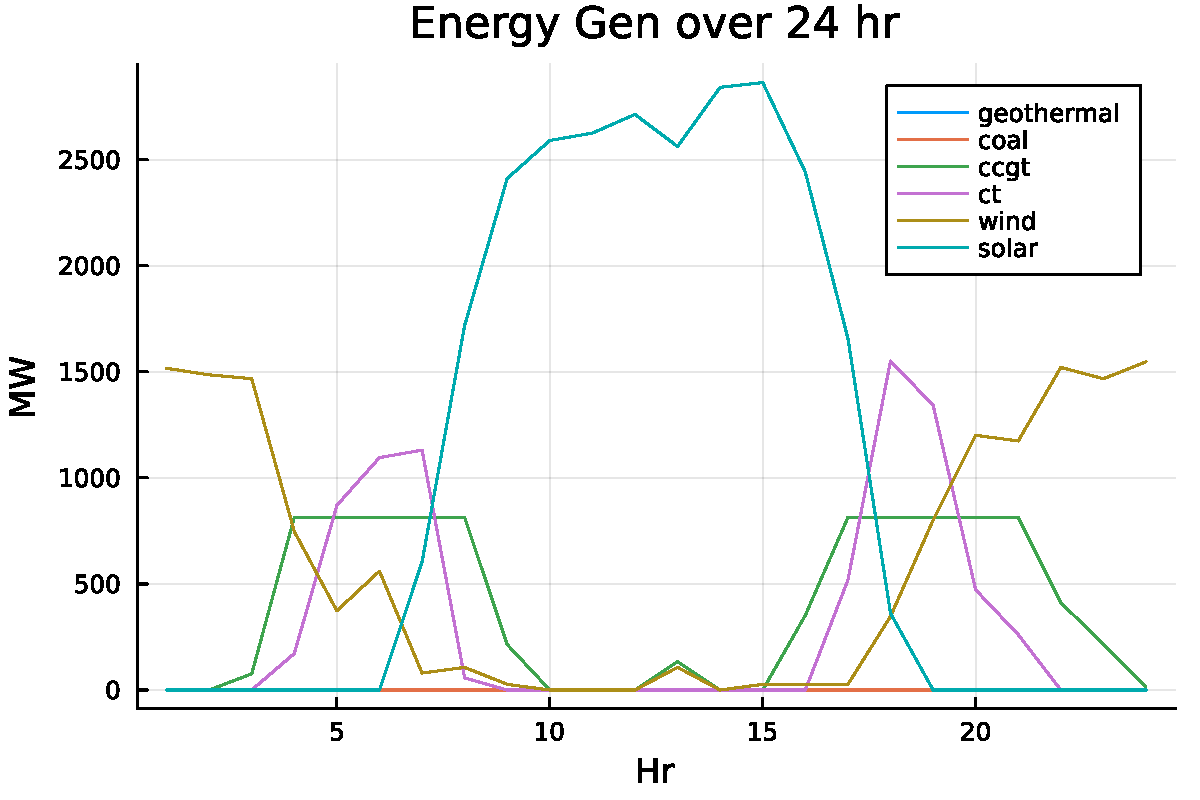
\includegraphics[width=\linewidth]{figures/solution-template_10_1.pdf}

\begin{lstlisting}
(*@\HLJLnB{julia>}@*) (*@\HLJLcs{{\#}}@*) (*@\HLJLcs{plot}@*) (*@\HLJLcs{stacked}@*) (*@\HLJLcs{area}@*) (*@\HLJLcs{plot}@*)
       (*@\HLJLnf{areaplot}@*)(*@\HLJLp{(}@*)(*@\HLJLn{loads}@*)(*@\HLJLoB{{\textquotesingle}}@*)(*@\HLJLp{,}@*) (*@\HLJLn{label}@*)(*@\HLJLoB{=}@*)(*@\HLJLnf{permutedims}@*)(*@\HLJLp{([}@*)(*@\HLJLs{"{}geothermal"{}}@*)(*@\HLJLp{,}@*)(*@\HLJLs{"{}coal"{}}@*)(*@\HLJLp{,}@*)(*@\HLJLs{"{}ccgt"{}}@*)(*@\HLJLp{,}@*)(*@\HLJLs{"{}ct"{}}@*)(*@\HLJLp{,}@*)(*@\HLJLs{"{}wind"{}}@*)(*@\HLJLp{,}@*)(*@\HLJLs{"{}solar"{}}@*)(*@\HLJLp{]),}@*) (*@\HLJLn{title}@*)(*@\HLJLoB{=}@*)(*@\HLJLs{"{}Energy}@*) (*@\HLJLs{Gen}@*) (*@\HLJLs{over}@*) (*@\HLJLs{24}@*) (*@\HLJLs{hr"{}}@*)(*@\HLJLp{,}@*) (*@\HLJLn{xlabel}@*)(*@\HLJLoB{=}@*)(*@\HLJLs{"{}Hr"{}}@*)(*@\HLJLp{,}@*) (*@\HLJLn{ylabel}@*)(*@\HLJLoB{=}@*)(*@\HLJLs{"{}MW"{}}@*))
\end{lstlisting}
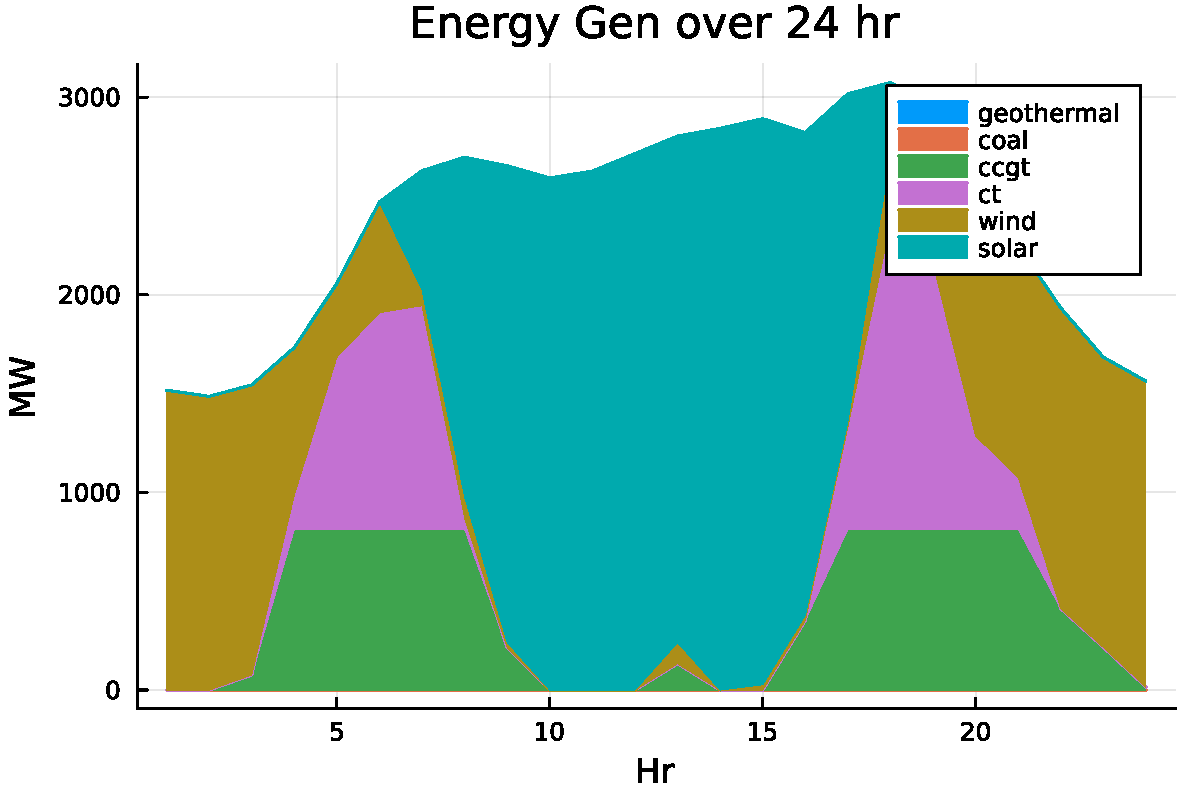
\includegraphics[width=\linewidth]{figures/solution-template_10_2.pdf}

Similar to before, solar energy is the main draw during the sunny hours of the day. During  the transitional hours, CCGT use decreases, CT increases, and wind increases.  Wind and CCGT are still the main contributors in the nighttime.

\subsection{Problem 2.5}

\begin{lstlisting}
(*@\HLJLnB{julia>}@*) (*@\HLJLcs{{\#}}@*) (*@\HLJLcs{create}@*) (*@\HLJLcs{new}@*) (*@\HLJLcs{model}@*)
       (*@\HLJLn{gencap3}@*) (*@\HLJLoB{=}@*) (*@\HLJLnf{Model}@*)(*@\HLJLp{(}@*)(*@\HLJLn{HiGHS}@*)(*@\HLJLoB{.}@*)(*@\HLJLn{Optimizer}@*)(*@\HLJLp{)}@*)
A JuMP Model
Feasibility problem with:
Variables: 0
Model mode: AUTOMATIC
CachingOptimizer state: EMPTY(*@{{\_}}@*)OPTIMIZER
Solver name: HiGHS

(*@\HLJLnB{julia>}@*) (*@\HLJLcs{{\#}}@*) (*@\HLJLcs{add}@*) (*@\HLJLcs{different}@*) (*@\HLJLcs{energy}@*) (*@\HLJLcs{gen}@*) (*@\HLJLcs{types}@*)
       (*@\HLJLn{generators}@*) (*@\HLJLoB{=}@*) (*@\HLJLp{[}@*)(*@\HLJLs{"{}geothermal"{}}@*)(*@\HLJLp{,}@*) (*@\HLJLs{"{}coal"{}}@*)(*@\HLJLp{,}@*) (*@\HLJLs{"{}ccgt"{}}@*)(*@\HLJLp{,}@*) (*@\HLJLs{"{}ct"{}}@*)(*@\HLJLp{,}@*) (*@\HLJLs{"{}wind"{}}@*)(*@\HLJLp{,}@*) (*@\HLJLs{"{}solar"{}}@*)(*@\HLJLp{];}@*)

(*@\HLJLnB{julia>}@*) (*@\HLJLcs{{\#}}@*) (*@\HLJLcs{variables}@*)
       (*@\HLJLn{G}@*) (*@\HLJLoB{=}@*) (*@\HLJLni{1}@*)(*@\HLJLoB{:}@*)(*@\HLJLnf{length}@*)(*@\HLJLp{(}@*)(*@\HLJLn{generators}@*)(*@\HLJLp{);}@*)

(*@\HLJLnB{julia>}@*) (*@\HLJLn{T}@*) (*@\HLJLoB{=}@*) (*@\HLJLni{1}@*)(*@\HLJLoB{:}@*)(*@\HLJLnf{length}@*)(*@\HLJLp{(}@*)(*@\HLJLn{hours}@*)(*@\HLJLp{);}@*)

(*@\HLJLnB{julia>}@*) (*@\HLJLnd{@variable}@*)(*@\HLJLp{(}@*)(*@\HLJLn{gencap3}@*)(*@\HLJLp{,}@*) (*@\HLJLn{x}@*)(*@\HLJLp{[}@*)(*@\HLJLn{G}@*)(*@\HLJLp{]}@*) (*@\HLJLoB{>=}@*) (*@\HLJLni{0}@*)(*@\HLJLp{);}@*)

(*@\HLJLnB{julia>}@*) (*@\HLJLnd{@variable}@*)(*@\HLJLp{(}@*)(*@\HLJLn{gencap3}@*)(*@\HLJLp{,}@*) (*@\HLJLn{y}@*)(*@\HLJLp{[}@*)(*@\HLJLn{G}@*)(*@\HLJLp{,}@*)(*@\HLJLn{T}@*)(*@\HLJLp{]}@*) (*@\HLJLoB{>=}@*) (*@\HLJLni{0}@*)(*@\HLJLp{);}@*)

(*@\HLJLnB{julia>}@*) (*@\HLJLnd{@variable}@*)(*@\HLJLp{(}@*)(*@\HLJLn{gencap3}@*)(*@\HLJLp{,}@*) (*@\HLJLn{nse}@*)(*@\HLJLp{[}@*)(*@\HLJLn{T}@*)(*@\HLJLp{]}@*) (*@\HLJLoB{>=}@*) (*@\HLJLni{0}@*)(*@\HLJLp{);}@*)

(*@\HLJLnB{julia>}@*) (*@\HLJLcs{{\#}}@*) (*@\HLJLcs{create}@*) (*@\HLJLcs{objective}@*) (*@\HLJLcs{function}@*)
       (*@\HLJLnd{@objective}@*)(*@\HLJLp{(}@*)(*@\HLJLn{gencap3}@*)(*@\HLJLp{,}@*) (*@\HLJLn{Min}@*)(*@\HLJLp{,}@*) (*@\HLJLn{investment{\_}cost}@*)(*@\HLJLoB{{\textquotesingle}*}@*)(*@\HLJLn{x}@*) (*@\HLJLoB{+}@*) (*@\HLJLnf{sum}@*)(*@\HLJLp{(}@*)(*@\HLJLn{op{\_}cost}@*)(*@\HLJLoB{.*}@*)(*@\HLJLn{y}@*)(*@\HLJLp{)}@*)(*@\HLJLoB{*}@*)(*@\HLJLni{365}@*) (*@\HLJLoB{+}@*) (*@\HLJLni{1000}@*)(*@\HLJLoB{*}@*)(*@\HLJLnf{sum}@*)(*@\HLJLp{(}@*)(*@\HLJLn{nse}@*)(*@\HLJLp{))}@*)(*@\HLJLoB{*}@*)(*@\HLJLni{365}@*)(*@\HLJLp{;}@*)

(*@\HLJLnB{julia>}@*) (*@\HLJLcs{{\#}}@*) (*@\HLJLcs{generators}@*) (*@\HLJLcs{cannot}@*) (*@\HLJLcs{produce}@*) (*@\HLJLcs{more}@*) (*@\HLJLcs{than}@*) (*@\HLJLcs{their}@*) (*@\HLJLcs{installed}@*) (*@\HLJLcs{capacity}@*) (*@\HLJLcs{and}@*) (*@\HLJLcs{availability}@*)
       (*@\HLJLn{avail}@*) (*@\HLJLoB{=}@*) (*@\HLJLnf{zeros}@*)(*@\HLJLp{(}@*)(*@\HLJLnf{length}@*)(*@\HLJLp{(}@*)(*@\HLJLn{G}@*)(*@\HLJLp{),}@*) (*@\HLJLnf{length}@*)(*@\HLJLp{(}@*)(*@\HLJLn{T}@*)(*@\HLJLp{));}@*)

(*@\HLJLnB{julia>}@*) (*@\HLJLn{avail}@*)(*@\HLJLp{[}@*)(*@\HLJLni{1}@*)(*@\HLJLp{,}@*)(*@\HLJLoB{:}@*)(*@\HLJLp{]}@*) (*@\HLJLoB{=}@*) (*@\HLJLn{thermal{\_}cf}@*)(*@\HLJLp{[}@*)(*@\HLJLni{1}@*)(*@\HLJLp{]}@*)(*@\HLJLoB{*}@*)(*@\HLJLnf{ones}@*)(*@\HLJLp{(}@*)(*@\HLJLnf{length}@*)(*@\HLJLp{(}@*)(*@\HLJLn{T}@*)(*@\HLJLp{));}@*)

(*@\HLJLnB{julia>}@*) (*@\HLJLn{avail}@*)(*@\HLJLp{[}@*)(*@\HLJLni{2}@*)(*@\HLJLp{,}@*)(*@\HLJLoB{:}@*)(*@\HLJLp{]}@*) (*@\HLJLoB{=}@*) (*@\HLJLn{thermal{\_}cf}@*)(*@\HLJLp{[}@*)(*@\HLJLni{2}@*)(*@\HLJLp{]}@*)(*@\HLJLoB{*}@*)(*@\HLJLnf{ones}@*)(*@\HLJLp{(}@*)(*@\HLJLnf{length}@*)(*@\HLJLp{(}@*)(*@\HLJLn{T}@*)(*@\HLJLp{));}@*)

(*@\HLJLnB{julia>}@*) (*@\HLJLn{avail}@*)(*@\HLJLp{[}@*)(*@\HLJLni{3}@*)(*@\HLJLp{,}@*)(*@\HLJLoB{:}@*)(*@\HLJLp{]}@*) (*@\HLJLoB{=}@*) (*@\HLJLn{thermal{\_}cf}@*)(*@\HLJLp{[}@*)(*@\HLJLni{3}@*)(*@\HLJLp{]}@*)(*@\HLJLoB{*}@*)(*@\HLJLnf{ones}@*)(*@\HLJLp{(}@*)(*@\HLJLnf{length}@*)(*@\HLJLp{(}@*)(*@\HLJLn{T}@*)(*@\HLJLp{));}@*)

(*@\HLJLnB{julia>}@*) (*@\HLJLn{avail}@*)(*@\HLJLp{[}@*)(*@\HLJLni{4}@*)(*@\HLJLp{,}@*)(*@\HLJLoB{:}@*)(*@\HLJLp{]}@*) (*@\HLJLoB{=}@*) (*@\HLJLn{thermal{\_}cf}@*)(*@\HLJLp{[}@*)(*@\HLJLni{4}@*)(*@\HLJLp{]}@*)(*@\HLJLoB{*}@*)(*@\HLJLnf{ones}@*)(*@\HLJLp{(}@*)(*@\HLJLnf{length}@*)(*@\HLJLp{(}@*)(*@\HLJLn{T}@*)(*@\HLJLp{));}@*)

(*@\HLJLnB{julia>}@*) (*@\HLJLn{avail}@*)(*@\HLJLp{[}@*)(*@\HLJLni{5}@*)(*@\HLJLp{,}@*)(*@\HLJLoB{:}@*)(*@\HLJLp{]}@*) (*@\HLJLoB{=}@*) (*@\HLJLn{wind{\_}cf}@*)(*@\HLJLp{;}@*)

(*@\HLJLnB{julia>}@*) (*@\HLJLn{avail}@*)(*@\HLJLp{[}@*)(*@\HLJLni{6}@*)(*@\HLJLp{,}@*)(*@\HLJLoB{:}@*)(*@\HLJLp{]}@*) (*@\HLJLoB{=}@*) (*@\HLJLn{solar{\_}cf}@*)(*@\HLJLp{;}@*)

(*@\HLJLnB{julia>}@*) (*@\HLJLnd{@constraint}@*)(*@\HLJLp{(}@*)(*@\HLJLn{gencap3}@*)(*@\HLJLp{,}@*) (*@\HLJLn{availability}@*)(*@\HLJLp{[}@*)(*@\HLJLn{g}@*) (*@\HLJLkp{in}@*) (*@\HLJLn{G}@*)(*@\HLJLp{,}@*) (*@\HLJLn{t}@*) (*@\HLJLkp{in}@*) (*@\HLJLn{T}@*)(*@\HLJLp{],}@*) (*@\HLJLn{y}@*)(*@\HLJLp{[}@*)(*@\HLJLn{g}@*)(*@\HLJLp{,}@*) (*@\HLJLn{t}@*)(*@\HLJLp{]}@*) (*@\HLJLoB{<=}@*) (*@\HLJLn{avail}@*)(*@\HLJLp{[}@*)(*@\HLJLn{g}@*)(*@\HLJLp{,}@*) (*@\HLJLn{t}@*)(*@\HLJLp{]}@*) (*@\HLJLoB{*}@*) (*@\HLJLn{x}@*)(*@\HLJLp{[}@*)(*@\HLJLn{g}@*)(*@\HLJLp{]);}@*)

(*@\HLJLnB{julia>}@*) (*@\HLJLcs{{\#}}@*) (*@\HLJLcs{need}@*) (*@\HLJLcs{to}@*) (*@\HLJLcs{serve}@*) (*@\HLJLcs{load}@*) (*@\HLJLcs{during}@*) (*@\HLJLcs{each}@*) (*@\HLJLcs{time}@*) (*@\HLJLcs{period}@*)
       (*@\HLJLnd{@constraint}@*)(*@\HLJLp{(}@*)(*@\HLJLn{gencap3}@*)(*@\HLJLp{,}@*) (*@\HLJLn{load}@*)(*@\HLJLp{[}@*)(*@\HLJLn{t}@*) (*@\HLJLkp{in}@*) (*@\HLJLn{T}@*)(*@\HLJLp{],}@*) (*@\HLJLnf{sum}@*)(*@\HLJLp{(}@*)(*@\HLJLn{y}@*)(*@\HLJLp{[}@*)(*@\HLJLoB{:}@*)(*@\HLJLp{,}@*)(*@\HLJLn{t}@*)(*@\HLJLp{])}@*) (*@\HLJLoB{+}@*) (*@\HLJLn{nse}@*)(*@\HLJLp{[}@*)(*@\HLJLn{t}@*)(*@\HLJLp{]}@*) (*@\HLJLoB{==}@*) (*@\HLJLn{demand}@*)(*@\HLJLp{[}@*)(*@\HLJLn{t}@*)(*@\HLJLp{]);}@*)

(*@\HLJLnB{julia>}@*) (*@\HLJLcs{{\#}}@*) (*@\HLJLcs{new}@*) (*@\HLJLcs{emissions}@*) (*@\HLJLcs{constraint}@*)
       (*@\HLJLnd{@constraint}@*)(*@\HLJLp{(}@*)(*@\HLJLn{gencap3}@*)(*@\HLJLp{,}@*) (*@\HLJLn{emissions}@*)(*@\HLJLp{[}@*)(*@\HLJLn{g}@*) (*@\HLJLkp{in}@*) (*@\HLJLn{G}@*)(*@\HLJLp{],}@*) (*@\HLJLp{(}@*)(*@\HLJLnf{sum}@*)(*@\HLJLp{(}@*)(*@\HLJLn{y}@*)(*@\HLJLp{[}@*)(*@\HLJLn{g}@*)(*@\HLJLp{,}@*)(*@\HLJLoB{:}@*)(*@\HLJLp{])}@*)(*@\HLJLoB{*}@*)(*@\HLJLn{co2{\_}emissions}@*)(*@\HLJLp{[}@*)(*@\HLJLn{g}@*)(*@\HLJLp{]}@*)(*@\HLJLoB{*}@*)(*@\HLJLni{365}@*)(*@\HLJLp{)}@*) (*@\HLJLoB{<=}@*) (*@\HLJLnfB{1.501}@*)(*@\HLJLoB{*}@*)(*@\HLJLni{10}@*)(*@\HLJLoB{{\textasciicircum}}@*)(*@\HLJLni{6}@*)(*@\HLJLp{);}@*)

(*@\HLJLnB{julia>}@*) (*@\HLJLcs{{\#}}@*) (*@\HLJLcs{non-negativity}@*) (*@\HLJLcs{established}@*) (*@\HLJLcs{when}@*) (*@\HLJLcs{the}@*) (*@\HLJLcs{variables}@*) (*@\HLJLcs{were}@*) (*@\HLJLcs{created}@*)
       
       (*@\HLJLcs{{\#}}@*) (*@\HLJLcs{optimize}@*) (*@\HLJLcs{model}@*)
       (*@\HLJLnf{optimize!}@*)(*@\HLJLp{(}@*)(*@\HLJLn{gencap3}@*)(*@\HLJLp{)}@*)
Presolving model
159 rows, 162 cols, 492 nonzeros
84 rows, 87 cols, 204 nonzeros
Presolve : Reductions: rows 84(-90); columns 87(-87); elements 204(-312)
Solving the presolved LP
Using EKK dual simplex solver - serial
  Iteration        Objective     Infeasibilities num(sum)
          0     0.0000000000e+00 Pr: 24(60321.5) 0s
         84     5.7037000000e+07 Pr: 0(0) 0s
Solving the original LP from the solution after postsolve
Model   status      : Optimal
Simplex   iterations: 84
Objective value     :  5.7037000000e+07
HiGHS run time      :          0.00

(*@\HLJLnB{julia>}@*) (*@\HLJLnf{objective{\_}value}@*)(*@\HLJLp{(}@*)(*@\HLJLn{gencap3}@*)(*@\HLJLp{)}@*)
5.7037e7
\end{lstlisting}

This new emissions limit would save \$ 55,149.

\section{References}
Extracting JuMP results. Julia Discourse. https://discourse.julialang.org/t/extracting-jump-results/51429 

First Steps with DataFrames.jl. DataFrames.jl Documentation. https://dataframes.juliadata.org/stable/man/basics/\#First-Steps-with-DataFrames.jl 

Multiple labels must be in a row vector. Plots.jl Issues. https://github.com/JuliaPlots/Plots.jl/issues/901 



\end{document}